
The Chang'E-4 mission, initiated in 2019, coincided with a period of solar minimum characterized by a scarcity of \ac{SEP} events. However, as sun stepping into the increase phase of new \ac{SC} and becoming more active than the solar minimum, solar activity has intensified, and consequencely, a growing number of \acs{SEP}, including prolonged-duration and high-intensity one, have been observed to reach the lunar surface and have been detected by the \ac{LND} on the lunar far-side surface. For example, Guo et al. (2023) recently reported the first \ac{GLE} of \ac{SC} 25, which were concurrently detected by instruments deployed on the Moon, Earth, Mars and also by \ac{SolO} as well as \ac{PSP} [citation of other studies]. It is noteworthy that \ac{LND} was switched on during the the decay phase of this events, hence missed the onset phase of the event. Even so, it still improves our understanding of potential radiaton risk that caused by those extreme \ac{SEP} events on the planetary surface.
In the appendix section of this thesis, a comprehensive list of \ac{SEP} events detected by the \ac{LND} on the lunar far-side surface between 2019 and 2023 is provided, further emphsizing on \ac{LND}'s contribution to the study of \acs{SEP}.


The \ac{SEP} event happened on May 6, 2019 is the first \ac{SEP} event that have was detected on the lunar surface in the past decade, according to our knowledge. 
This \ac{SEP} event is associated with an M-class flare originating from solar active region (AR12470) which is located on the eastern hemisphere and is more than 110 degrees away from the Earth's magnetic footpoint on the solar surface. The remote-sensing observations conducted by the \ac{SOHO}/\ac{LASCO} and \ac{STEREO} revealed the presence of a slow, narrow, and westward moving \ac{CME}. 
Though those \acs{SEP} cause negligible radiation dose due to its weak intensity and lower peak energy, it is still an interesting event and worth studying due to the following two reasons.
The primary objective of this study is to utilize the first \ac{SEP} event observed by \ac{LND} to validate the data products produced during \ac{SEP} occurrences and assess the instrument's performance under such conditions. By cross calibrating the proton measurements between \ac{LND} and other already existed particle instruments at the first lagrange point, specifically the \ac{EPHIN} onboard \ac{SOHO} and \ac{ACE}/\ac{EPAM}, we conclude that \ac{LND} provide reliable solar energetic proton measurement with high time resolution of one minute.
%For sure LND is outside of the mangetosphere, but still that is one of the thing worth to look at. How the SEP propogarting across the magnetosphere and arrive the magnetosphere tails.
Additionally, we aim to investigate the extensive spatial distribution of this \ac{SEP}. Several mechanisms could be invovled in the process of the particle traversal across considerable distance in the so-call wide spread \acs{SEP}. Combined the in-site and remote-sensing measurement, we try to found out what kind release and propagation mechanism are involved in this event.

The following article is reproduced from \textcite{Xu2020ApJ} by permission of the AAS:\\

\noindent\pubcite{Xu2020ApJ}\\
\strut\hfill Own contribution: 80\%

\newpage
\newcounter{includepdfpageAPJLTwenty}

\addtocounter{section}{1}
\setcounter{section}{1} 
% \phantomsection
% \addcontentsline{toc}{section}{\arabic{chapter}.\arabic{section} First Solar Energetic Particles Measured on the Lunar Far-side(Publication ApJ Letter 2020)}
%
\phantomsection
\addcontentsline{toc}{section}{\arabic{chapter}.\arabic{section} Introduction}
\label{sec:paper_xu2020}
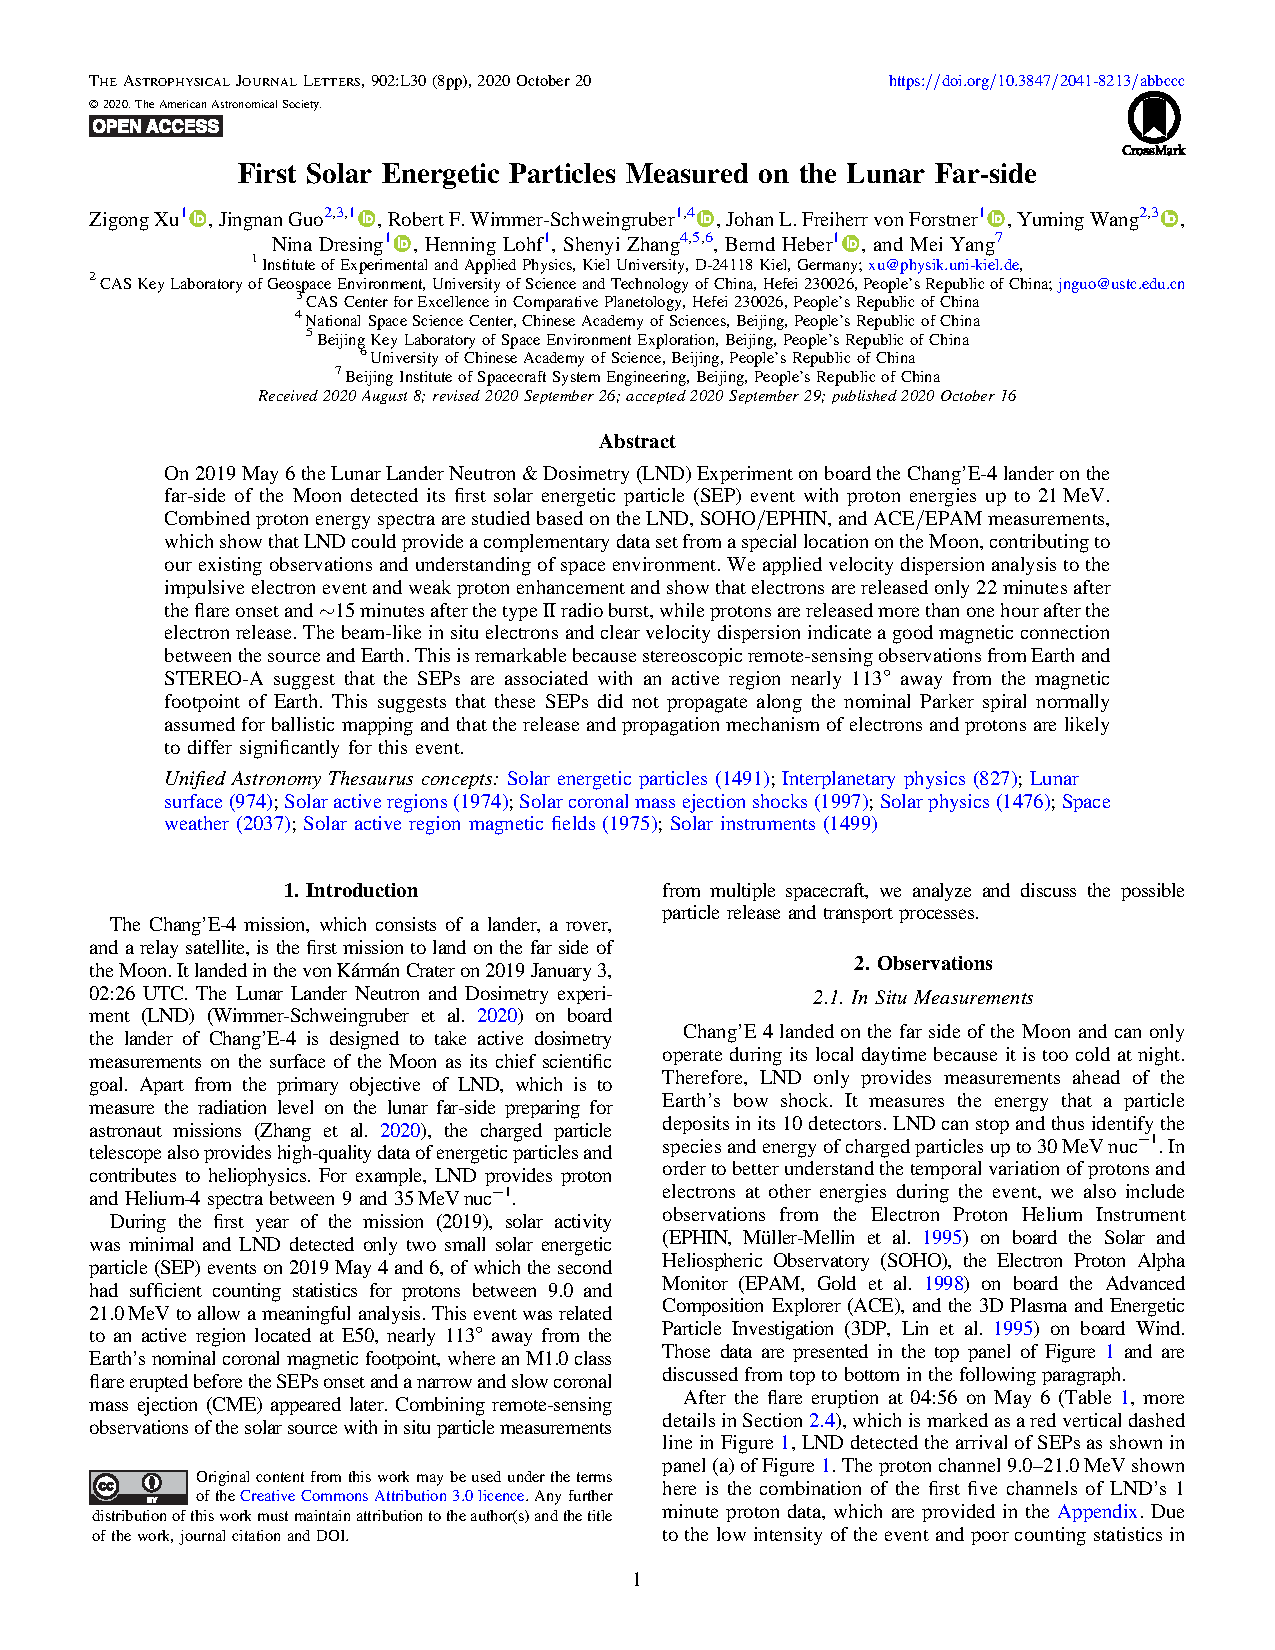
\includepdf[pages={1}, link, linkname=paper_xu2020, scale=.9, pagecommand={\refstepcounter{includepdfpageAPJLTwenty}\label{paper_xu2020.\theincludepdfpageAPJLTwenty}}]{publications/Xu_et_al_2020_ApJL.pdf}
%
\addtocounter{section}{1} 
\phantomsection
\addcontentsline{toc}{section}{\arabic{chapter}.\arabic{section} Observations}
\includepdf[pages={2-4}, link, linkname=paper_xu2020, scale=.9, pagecommand={\refstepcounter{includepdfpageAPJLTwenty}\label{paper_xu2020.\theincludepdfpageAPJLTwenty}}]{publications/Xu_et_al_2020_ApJL.pdf}
%
\addtocounter{section}{1} 
\phantomsection
\addcontentsline{toc}{section}{\arabic{chapter}.\arabic{section} Summary and Discussion}
\includepdf[pages={5-6}, link, linkname=paper_xu2020, scale=.9, pagecommand={\refstepcounter{includepdfpageAPJLTwenty}\label{paper_xu2020.\theincludepdfpageAPJLTwenty}}]{publications/Xu_et_al_2020_ApJL.pdf}
%
\addtocounter{section}{1} 
\phantomsection
\addcontentsline{toc}{section}{\arabic{chapter}.\arabic{section} Appendix}
\includepdf[pages={7}, link, linkname=paper_xu2020, scale=.9, pagecommand={\refstepcounter{includepdfpageAPJLTwenty}\label{paper_xu2020.\theincludepdfpageAPJLTwenty}}]{publications/Xu_et_al_2020_ApJL.pdf}
%
\addtocounter{section}{1} 
\phantomsection
\addcontentsline{toc}{section}{\arabic{chapter}.\arabic{section} References}
\includepdf[pages={8}, link, linkname=paper_xu2020, scale=.9, pagecommand={\refstepcounter{includepdfpageAPJLTwenty}\label{paper_xu2020.\theincludepdfpageAPJLTwenty}}]{publications/Xu_et_al_2020_ApJL.pdf}
